\documentclass[11pt]{article}

\newcommand{\yourname}{Zerun Tian}
\newcommand{\yourcollaborators}{}

\def\comments{0}

\def\comments{0}
\setlength{\parindent}{0 in}
\setlength{\parskip}{0.1in}

%format and packages

%\usepackage{algorithm, algorithmic}
\usepackage[noend]{algpseudocode}
\usepackage{amsmath, amssymb, amsthm}
\usepackage{enumerate}
\usepackage{enumitem}
\usepackage{framed}
\usepackage{verbatim}
\usepackage[margin=1.0in]{geometry}
\usepackage{microtype}
\usepackage{kpfonts}
\usepackage{palatino}
	\DeclareMathAlphabet{\mathtt}{OT1}{cmtt}{m}{n}
	\SetMathAlphabet{\mathtt}{bold}{OT1}{cmtt}{bx}{n}
	\DeclareMathAlphabet{\mathsf}{OT1}{cmss}{m}{n}
	\SetMathAlphabet{\mathsf}{bold}{OT1}{cmss}{bx}{n}
	\renewcommand*\ttdefault{cmtt}
	\renewcommand*\sfdefault{cmss}
	\renewcommand{\baselinestretch}{1.06}
\usepackage[usenames,dvipsnames]{xcolor}
\definecolor{DarkGreen}{rgb}{0.15,0.5,0.15}
\definecolor{DarkRed}{rgb}{0.6,0.2,0.2}
\definecolor{DarkBlue}{rgb}{0.2,0.2,0.6}
\definecolor{DarkPurple}{rgb}{0.4,0.2,0.4}
\usepackage[pdftex]{hyperref}
\hypersetup{
	linktocpage=true,
	colorlinks=true,				% false: boxed links; true: colored links
	linkcolor=DarkBlue,		% color of internal links
	citecolor=DarkBlue,	% color of links to bibliography
	urlcolor=DarkBlue,		% color of external links
}

\usepackage{graphicx}
\graphicspath{ {./} }

%enclosure macros
\newcommand{\paren}[1]{\ensuremath{\left( {#1} \right)}}
\newcommand{\bracket}[1]{\ensuremath{\left\{ {#1} \right\}}}
\renewcommand{\sb}[1]{\ensuremath{\left[ {#1} \right\]}}
\newcommand{\ab}[1]{\ensuremath{\left\langle {#1} \right\rangle}}

%probability macros
\newcommand{\ex}[2]{{\ifx&#1& \mathbb{E} \else \underset{#1}{\mathbb{E}} \fi \left[#2\right]}}
\newcommand{\pr}[2]{{\ifx&#1& \mathbb{P} \else \underset{#1}{\mathbb{P}} \fi \left[#2\right]}}
\newcommand{\var}[2]{{\ifx&#1& \mathrm{Var} \else \underset{#1}{\mathrm{Var}} \fi \left[#2\right]}}

%useful CS macros
\newcommand{\poly}{\mathrm{poly}}
\newcommand{\polylog}{\mathrm{polylog}}
\newcommand{\zo}{\{0,1\}}
\newcommand{\pmo}{\{\pm1\}}
\newcommand{\getsr}{\gets_{\mbox{\tiny R}}}
\newcommand{\card}[1]{\left| #1 \right|}
\newcommand{\set}[1]{\left\{#1\right\}}
\newcommand{\negl}{\mathrm{negl}}
\newcommand{\eps}{\varepsilon}
\DeclareMathOperator*{\argmin}{arg\,min}
\DeclareMathOperator*{\argmax}{arg\,max}
\newcommand{\eqand}{\qquad \textrm{and} \qquad}
\newcommand{\ind}[1]{\mathbb{I}\{#1\}}
\newcommand{\sslash}{\ensuremath{\mathbin{/\mkern-3mu/}}}

%mathbb
\newcommand{\N}{\mathbb{N}}
\newcommand{\R}{\mathbb{R}}
\newcommand{\Z}{\mathbb{Z}}
%mathcal
\newcommand{\cA}{\mathcal{A}}
\newcommand{\cB}{\mathcal{B}}
\newcommand{\cC}{\mathcal{C}}
\newcommand{\cD}{\mathcal{D}}
\newcommand{\cE}{\mathcal{E}}
\newcommand{\cF}{\mathcal{F}}
\newcommand{\cL}{\mathcal{L}}
\newcommand{\cM}{\mathcal{M}}
\newcommand{\cO}{\mathcal{O}}
\newcommand{\cP}{\mathcal{P}}
\newcommand{\cQ}{\mathcal{Q}}
\newcommand{\cR}{\mathcal{R}}
\newcommand{\cS}{\mathcal{S}}
\newcommand{\cU}{\mathcal{U}}
\newcommand{\cV}{\mathcal{V}}
\newcommand{\cW}{\mathcal{W}}
\newcommand{\cX}{\mathcal{X}}
\newcommand{\cY}{\mathcal{Y}}
\newcommand{\cZ}{\mathcal{Z}}

%theorem macros
\newtheorem{thm}{Theorem}
\newtheorem{lem}[thm]{Lemma}
\newtheorem{fact}[thm]{Fact}
\newtheorem{clm}[thm]{Claim}
\newtheorem{rem}[thm]{Remark}
\newtheorem{coro}[thm]{Corollary}
\newtheorem{prop}[thm]{Proposition}
\newtheorem{conj}[thm]{Conjecture}

\theoremstyle{definition}
\newtheorem{defn}[thm]{Definition}


\newcommand{\instructor}{Virgil Pavlu}
\newcommand{\hwnum}{5}
\newcommand{\hwdue}{Wednesday, May 20 at 11:59pm via \href{https://gradescope.com/courses/229309}{Gradescope}}

\theoremstyle{theorem}
\newtheorem{prob}{}
\newtheorem{sol}{Solution}

\definecolor{cit}{rgb}{0.05,0.2,0.45} 
\newcommand{\solution}{\medskip\noindent{\color{DarkBlue}\textbf{Solution:}}}

\begin{document}
{\Large 
\begin{center}{CS5800: Algorithms} --- Spring '21 --- \instructor \end{center}}
{\large
\vspace{10pt}
\noindent Homework~\hwnum \vspace{2pt}\\
Submit via \href{https://www.gradescope.com/courses/232127}{Gradescope}}

\bigskip
{\large \noindent Name: \yourname }

{\large \noindent Collaborators: \yourcollaborators}

\vspace{15pt}

{\large \noindent Instructions:}

\begin{itemize}

\item Make sure to put your name on the first page.  If you are using the \LaTeX~template we provided, then you can make sure it appears by filling in the \texttt{yourname} command.

\item Please review the grading policy outlined in the course information page.

\item You must also write down with whom you worked on the assignment.  If this changes from problem to problem, then you should write down this information separately with each problem.

\item Problem numbers (like Exercise 3.1-1) are corresponding to CLRS $3^{rd}$ edition.  While the  $2^{nd}$ edition  has  similar  problems  with  similar  numbers,  the  actual  exercises  and their solutions are different, so make sure you are using the $3^{rd}$ edition.

\end{itemize}

%%% Problem 1 %%%
\newpage
\begin{prob} \textbf{(15 points)} Exercise 15.2-1.
\end{prob}
Find an optimal parenthesization of a matrix-chain product whose sequence of dimensions is $[5, 10, 3, 12, 5, 50, 6]$.

\solution

To solve this problem with dynamic programming, we use the following five steps.
\begin{enumerate}[label=(\arabic*)]
\item Characterize the optimal solution:

Suppose an optimal solution parenthesizes $A_iA_{i+1}...A_j$ by splitting between $A_k$ and $A_{k+1}$. We claim that, for subchains $A_i...A_k$ and $A_{k+1}...A_j$, they have optimal parenthesization, respectively. If any of the subchains had an even better parenthesization, it could replace the existing one and get a smaller number of scalar multiplications overall. This contradicts that our given solution is optimal, so our claim has to be correct.

\item Define the recurrence of the objective:

\[
C[i, j] = 
\begin{cases}
  0 												&\mbox{if } i = j \\
  \text{min}_{i \le k < j} \{C[i, k] + C[k+1, j] + p_{i-1} p_k p_j\} 	&\mbox{if } i < j 
\end{cases}
\]
We use $C[i, j]$ to denote the number of scalar multiplications for $A_iA_{i+1}...A_j$. For $i = j$, there is no multiplication to be performed. For $i < j$, we search for a $k$ between $i$ (inclusive) and $j$ (exclusive) such that the split yields the minimum number of scalar multiplications considering the optimal solution to subchain $C[i, k]$ and $C[k+1, j]$ plus $p_{i-1}p_kp_j$, which is the number of multiplications required for multiplying the two resulting matrices.

\item Compute the value of an optimal solution bottom-up:

We refer to the pseudocode $\textproc{\textsc{Matrix-Chain-Order}}$ on page 375 of CLRS.

\item Trace the optimal solution from the computed information:

In the procedure above, we have a table $S$ that records the optimal split $k$ at each cell, i.e. splitting between index $k$ and $k+1$. By inspecting where the optimal split $k$ is at $S[1, n]$, we find the outermost split. Then, we continue find the splits at $S[1, k]$ and $S[k+1, n]$ to split the two subchains further. The pseudocode $\textproc{\textsc{Print-Optimal-Parens}}$ can be found on page 377 of CLRS.

\item Runtime and space requirements:

The nested loop runs in $O(n^3)$ time which denominates the runtime of $\textproc{\textsc{Matrix-Chain-Order}}$. In terms of space complexity, we have $O(n^2)$ because we use two tables $C$ and $S$ of size $n^2$. 
\end{enumerate}

 After implementing the algorithm in code, we see the following results with the given dimensions.
  
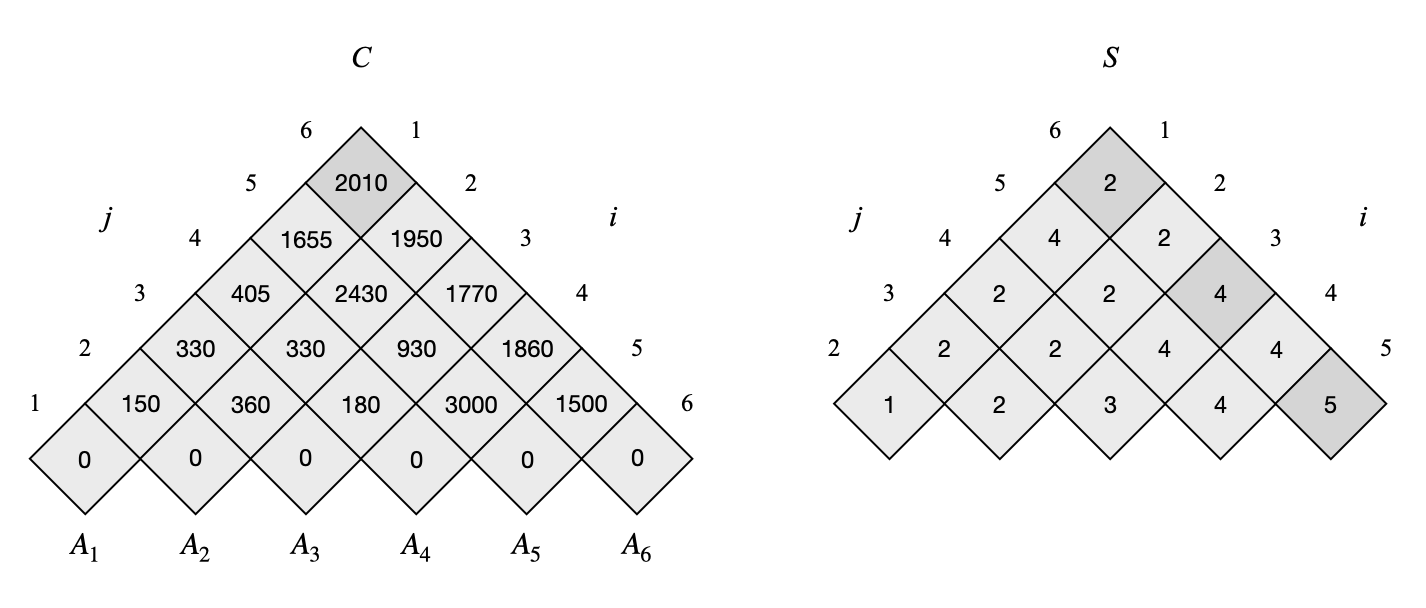
\includegraphics[scale=0.65]{hw5q1.png}

Notice that for $C[i, i]$ whose values are zeros, we are working with single matrices. They are $A_1$ of size 5 by 10, $A_2$ of size 10 by 3, and so on so forth. 

For $j - i = 1$, $C[i, j]$ cells can be trivially computed by multiplying $p_{i-1}p_ip_j$. For example, $C[1, 2] = p_0p_1p_2 = 5 \cdot 10 \cdot 3 = 150$. For $j - i = 2$ cells, there are two possible parenthesizations. For example, for $C[1, 3]$, we could have $A_1(A_2A_3)$ or $(A_1A_2)A_3$,
\[
C[1,3] = \text{min}
\begin{cases}
	C[1, 1] + C[2, 3] + p0p1p3= 0+360+5 \cdot 10 \cdot 12 =  960 \\
    	C[1, 2] + C[3, 3] + p0p2p3=150+0+5 \cdot 3 \cdot 12=150+180= \textbf{330}
\end{cases}
\]
The entry at $S[1, 3]$ is 2 because we just found splitting between 2 and 3 results in less scalar multiplications. So on so forth, we fill the tables. For the final cell $C[1, 6]$, we compare,
\[
C[1, 6] = \text{min}
\begin{cases}
	C[1, 1] + C[2, 6] + p_0p_1p_6 = 0 + 1950 + 5 \cdot 10 \cdot 6 = 2250 \\
	C[1, 2] + C[3, 6] + p_0p_2p_6 = 150 + 1770 + 5 \cdot 3 \cdot 6 = \textbf{2010} \\
	C[1, 3] + C[4, 6] + p_0p_3p_6 = 330 + 1840 + 5 \cdot 12 \cdot 6 = 2530 \\
	C[1, 4] + C[5, 6] + p_0p_4p_6 = 405 + 1500 + 5 \cdot 5 \cdot 6 = 2055 \\
	C[1, 5] + C[6, 6] + p_0p_5p_6 = 1655 + 0 + 5 \cdot 50 \cdot 6 = 3155 \\
\end{cases}
\]
and found that first splitting between 2 and 3 results in the least number of scalar multiplications.

By looking at $S$, we know that the outermost split is between 2 and 3, so we have $A_1A_2$ and $A_3...A_6$. Then, we find that the optimal split for $A_3...A_6$ is between 4 and 5. This gives us an optimal parenthesization: $((A_1 A_2) ((A_3 A_4) (A_5 A_6)))$.

Code is listed in the last page of the document.

%%% Problem 2 %%%
\newpage
\begin{prob} \textbf{(15 points)} Exercise 15.3-2.
\end{prob}
Draw the recursion tree for the \textproc{\textsc{Merge-Sort}} procedure from Section 2.3.1 on an array of 16 elements. Explain why memoization fails to speed up a good divide-and-conquer algorithm such as \textproc{\textsc{Merge-Sort}}.

\solution

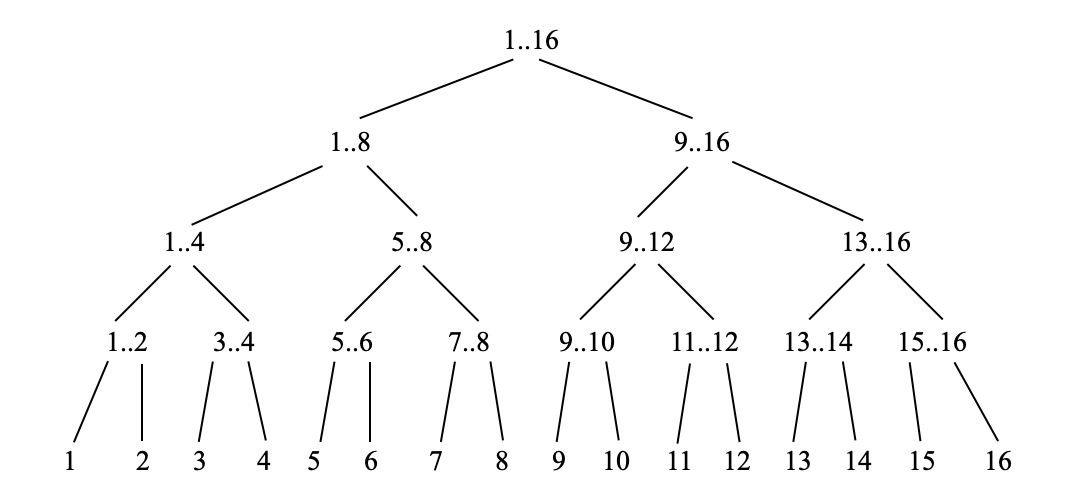
\includegraphics[scale=0.7]{hw5q2.png}

From the recursion tree, we observe that for each range of indices $b..e$, it only appeared once in the tree. \textproc{\textsc{Merge-Sort}} attempts to solve distinct inputs at every recursive call, which means there is no overlapping subproblem that needs to be stored to save computation time in a later call. Memoization in this problem even requires additional space.


%%% Problem 3 %%%
\newpage
\begin{prob} \textbf{(20 points)} Exercise 15.3-5.
\end{prob}
Suppose that in the rod-cutting problem of Section 15.1, we also had limit $l_i$ on the number of pieces of length $i$ that we are allowed to produce, for $i = 1, 2, ..., n$. Show that the optimal-substructure property described in Section 15.1 no longer holds.

\solution

The optimal-substructure property states that the optimal solution to the rod-cutting problem incorporates optimal solutions to related subproblems, which may solve independently. 

For example, prices for rods of different length are: $p_1 = 1$, $p_2 = 1$, $p_3 = 10$. Following the DP solution, a length-7 rod depends on optimal solutions to a length-3 rod and a length-4 rod. For the length-3 rod, we gain the maximum value when not cutting it. For the length-4 rod, we gain the maximum value when cutting it into pieces of length 3 and 1. Hence, by cutting the length-7 rod into two pieces of length 3 and one piece of length 1, we maximize the value: $10 + 10 + 1 = 21$. The optimal-substructure holds for the normal rod-cutting problem. 

However, if we restrict the maximum number of pieces of length $i$ that we can produce, we could not solve the subproblems independently. Using the same example and adding some limits: $l_1 = 10$, $l_2 = 10$, $l_3 = 1$, the above optimal solution does not apply because we can only produce one length-3 rod. The true optimal solution is cutting the length-7 rod into one length-3 and four length-1 pieces, which results in the value: 10 + 1 + 1 + 1 + 1 = 14. This contradicts the optimal solution of DP. In this case, an optimal solution can no longer depends on optimal solutions to subproblems.


%%% Problem 4.a %%%
\newpage
\begin{prob} \textbf{(20 points)} Problem 15-5.
\end{prob}

\begin{enumerate}[label=\alph*.]
\item Given two sequences $x[1..m]$ and $y[1..n]$ and set of transformation-operation costs. Describe a dynamic-programming algorithm for the edit distance problem and prints an optimal operation sequence. Analyze the running time and space requirements of your algorithm.

\solution

\begin{algorithmic}[1]
\Function{EditDistance}{$x$, $y$}
	\State $m = x$.length, $n = y$.length
	\State let $C[0..m, 0..n]$ and $S[0..m, 0..n]$ be new tables. \Comment{tables initializtion}
	\For {$i = 0$ to $m$}
		\State $C[i, 0] = \textproc{\textsc{cost}}(\text{delete}) \cdot i$
		\State $S[i, 0] = (i-1, 0)$
	\EndFor
	\For {$j = 0$ to $n$}
		\State $C[0, j] = \textproc{\textsc{cost}}(\text{insert}) \cdot j$
		\State $S[0, j] = (0, j-1)$
	\EndFor
	\State $S[0, 0] = (0, 0)$
	\For {$i = 1$ to $m$}
		\For {$j = 1$ to $n$}
			\State $\textit{minCost} =$ +inf
			\State $\textit{c1} = \textproc{\textsc{cost}}(\text{copy}) + C[i-1, j-1]$ \Comment {setting up the recurrence}
			\State $\textit{c2} = \textproc{\textsc{cost}}(\text{replace}) + C[i-1, j-1]$ 
			\State $\textit{c3} = \textproc{\textsc{cost}}(\text{delete}) + C[i-1, j]$ 
			\State $\textit{c4} = \textproc{\textsc{cost}}(\text{insert}) + C[i, j-1]$
			\State $\textit{c5} = \textproc{\textsc{cost}}(\text{twiddle}) + C[i-2, j-2]$
			\If {$x[i] == y[j]$ and $\textit{c1} < \textit{minCost}$} \Comment {finding an operation to minimize cost}
				\State $\textit{minCost} = \textit{c1}$
				\State $S[i, j] = (i - 1, j - 1)$
			\EndIf
			\If {$\textit{c2} < \textit{minCost}$}
				\State $\textit{minCost} = \textit{c2}$
				\State $S[i, j] = (i - 1, j - 1)$
			\EndIf
			\If {$\textit{c3} < \textit{minCost}$}
				\State $\textit{minCost} = \textit{c3}$
				\State $S[i, j] = (i - 1, j)$
			\EndIf
			\If {$\textit{c4} < \textit{minCost}$}
				\State $\textit{minCost} = \textit{c4}$
				\State $S[i, j] = (i, j-1)$
			\EndIf
			\If {$\textit{c5} < \textit{minCost}$ and $i > 1$ and $j > 1$ and $x[i] == y[j-1]$ and $x[i-1] == y[j]$}
				\State $\textit{minCost} = \textit{c5}$
				\State $S[i, j] = (i-2, j-2)$
			\EndIf
			\State $C[i, j] = \textit{minCost}$
		\EndFor
	\EndFor
	\State \textbf{return} $C$ and $S$
\EndFunction
\end{algorithmic}

We use $C[i, j]$ to record the edit distance from $x[1..i]$ to $y[1..j]$; we store a pair of indices $(p, q)$ at $S[i, j]$ such that they identify the prefixes $x[1..p]$ and $y[1..q]$ after which the current operation is applied. For every $i$ and $j$, we calculate its edit distance by finding the minimum cost among possible operations plus the edit distance of the subproblem prior to that operation. The recurrence of the objective is expressed in the above pseudocode from line 13 to 34.

With the resulting $C$ and $S$ tables, we are able to trace an optimal operation sequence by using the following procedure.

\begin{algorithmic}[1]
\Function{TraceOperations}{$x$, $y$, $S$}
	\State \textit{ops} $= []$
	\State $i = x$.length
	\State $j = y$.length
	\While {$i > 0$ and $j > 0$}
		\State $p, q = S[i, j]$ \Comment{backtrace the i, j to find the subproblem}
		\State \textit{di} $= i - p$
		\State \textit{dj} $= j - q$
		\If {\textit{di} $== 1$ and \textit{dj} $== 1$}
			\If {$x[i] == y[j]$}
				\State \textit{ops}.append("copy " + $x[i]$)	
			\Else
				\State \textit{ops}.append("replace by " + $y[j]$)	
			\EndIf
		\ElsIf {\textit{di} $== 1$ and \textit{dj} $== 0$}
			\State \textit{ops}.append("delete " + $x[i]$)
		\ElsIf {\textit{di} $== 0$ and \textit{dj} $== 1$}
			\State \textit{ops}.append("insert " + $y[i]$)
		\ElsIf {\textit{di} $== 2$ and \textit{dj} $== 2$}
			\State \textit{ops}.append("twiddle " + $x[i-1]$ + " and " + $x[i]$)
		\EndIf
		\State $i = p$
		\State $j = q$
	\EndWhile
	\For {\textit{op} in \textit{ops}.reversed}
		\State \textproc{\textsc{print}}(op)
	\EndFor
\EndFunction
\end{algorithmic}

The running time of \textproc{\textsc{EditDistance}} is $O(mn)$ because the number of operations within the doubly-nested loop at line 11 is constant. The function \textproc{\textsc{TraceOperations}} run in $O(m + n)$-time as how we backtrace the cells of table $S$. Overall, the DP algorithm runs in $O(mn)$-time. In terms of space, \textproc{\textsc{EditDistance}} takes $O(mn)$ primarily for the two tables $C$ and $S$. The function \textproc{\textsc{TraceOperations}} takes $O(m + n)$-space to keep track of the selected operations. Overall, the space complexity of the algorithm is $O(mn)$.

%%% Problem 4.b %%%
\newpage
\item Explain how to cast the problem of finding an optimal alignment as an edit distance problem using a subset of the transformation operations copy, replace, delete, insert, twiddle, and kill.

\solution

We are going to choose the subset: \{copy, replace, delete, insert\}. To formulate the alignment problem into an edit distance problem, we associate costs to operations such that the minimization of edit distance creates a well-matched and compact alignment. 

When we delete a character from $x$, we think of it as adding a space to $y$ at the corresponding spot for alignment. Similarly, when we insert a character to somewhere in $y$, we view it as adding a space to $x$ for alignment. In these cases, alignment receives a $-2$ score, so we want to reduce such cases by associating a \textbf{cost of 2} with \textbf{delete} and \textbf{insert} operations. Furthermore, a \textbf{replace} operation implies that $x_j \ne y_j$, which receives a $-1$ in terms of alignment score. In this case, we want a \textbf{cost of 1} to be associated with \textbf{replace}. Finally, a \textbf{copy} operation implies that $x_j == y_j$ which results in a $+1$ for alignment score, so we associate a \textbf{cost -1}. We can solve the alignment problem of sequence $x$ and $y$ using the edit distance algorithm with those specific values for those operations. Finally, we find the $\textit{optimal-alignment-score} = 0 - \textit{edit-distance}$.
\end{enumerate}


%%% Problem 5 %%%
\newpage
\begin{prob} \textbf{(30 points)} (Note:  you should decide to use Greedy or DP on this problem)

\noindent Prof.  Curly is planning a cross-country road-trip from Boston to Seattle on Interstate 90, and he needs to rent a car. ... Your algorithm or algorithms should output both the total cost of the trip and the various cities at which rental cars must be dropped off and/or picked up.
\end{prob}
\solution

Let's try to solve this using DP.
\begin{enumerate}[label=(\arabic*)]
\item Characterize the optimal solution:

Suppose we are given an optimal solution: $[c_1, c_2, ..., c_m]$ where $c_1$ is Boston, $c_m$ is Seattle, and $c_2$ .. $c_{m-1}$ are cities where the professor should rent new cars to achieve an overall minimum cost. If we split it at any $c_k$ for $1 < k < m$, $[c_1, ..., c_k]$ is an optimal solution to the subproblem of going from city $c_1$ to $c_k$. And, $[c_k, ..., c_m]$ is optimal to the subproblem of going from city $c_k$ to $c_m$. 

To show it is correct, we assume there exists a lower cost plan for a subproblem, so we could replace it in the given solution to achieve an overall lower cost. However, this means that the given solution is not optimal: a contradiction.

\item Define the recurrence of the objective:
\[
C[i, j] = 
\begin{cases}
  0 												&\mbox{if } i = j \\
  \text{min}\left\{T[i, j], \text{min}_{i < k < j} \{C[i, k] + C[k, j]\} \right\} 		&\mbox{if } i < j 
\end{cases}
\]
We use $C[i, j]$ to denote the minimum cost possible to travel from the city $i$ to the city $j$. Because we don't consider backtrack, we omit cases of $i > j$. When $i < j$, the minimum cost is either going directly from city $i$ to $j$ or stopping at some city $k$ that minimizes $C[i, k] + C[k, j]$. 
 
 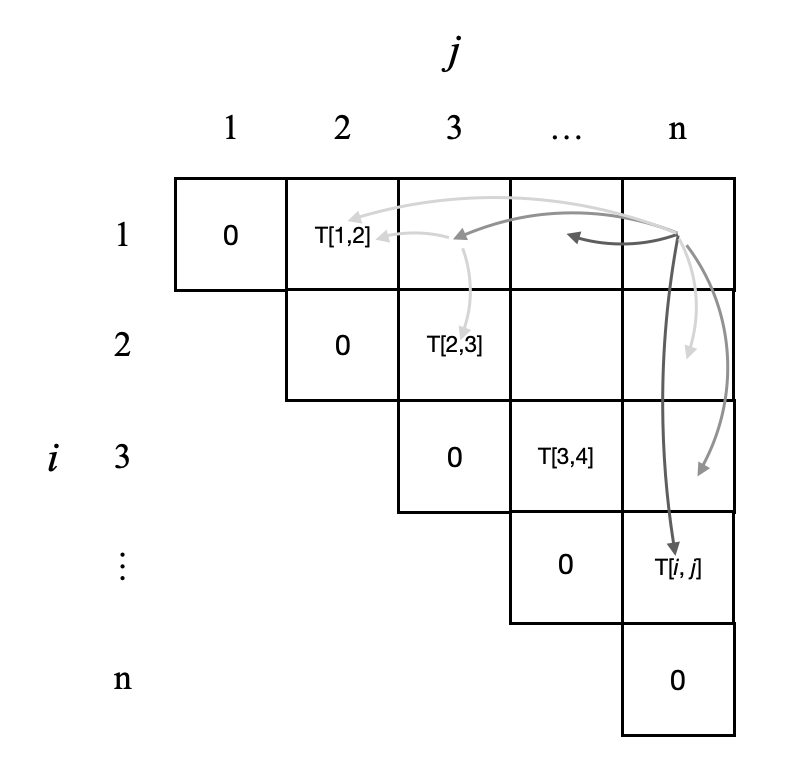
\includegraphics[scale=0.65]{hw5q5.png}
 
\item Compute the value of an optimal solution bottom-up:

\begin{algorithmic}[1]
\Function{PlanRentalCars}{$T$}
	\State let $C[1..n, 1..n]$, $S[1..n, 1..n]$ be new tables of zeros \Comment {tables initialization}
	\For {$i = 1$ to $n$}
		\For {$j = i + 1$ to $n$}
			\State $p = j - i - 1$
			\State $q = j$
			\State \textit{minCost } $= T[p, q]$ \Comment{setting up the recurrence}
			\State $S[p, q] = p$
			\For {$k = p + 1$ to $q - 1$}
				\State \textit{cost} $= C[p, k] + C[k, q]$
				\If {\textit{cost} $<$ \textit{minCost}}
					\State \textit{minCost} $ = $ \textit{cost}
					\State $S[p, q] = k$
				\EndIf 
				\State $C[p, q] = $ \textit{minCost}
			\EndFor
		\EndFor
	\EndFor
	\State \textbf{return} $C$, $S$
\EndFunction
\end{algorithmic}

\item Trace the optimal solution from the computed information:
\begin{algorithmic}[1]
\Function{TraceSolution}{\textit{cities}, $C$, $S$}
	\State $n =$ len$(\textit{cities})$
	\State $e = n$ \Comment{the index of ending city}
	\State $b = S[1][e]$ \Comment{the index of beginning city}
	\State \textproc{\textsc{Print}}("Total cost is " + $C[1, e]$)
	\State \textit{plan} $= \{1, e\}$ \Comment{store a set of indices of cities that made to the final plan}
	\While {$b \ne 1$} \Comment{continue unless the beginning city is Boston at index 1}
		\State $\textit{tmp} = b$
		\State $b = S[\textit{tmp}][e]$
		\State $e = tmp$
		\State $\textit{plan}.\textit{add}(e)$	\Comment{\textit{plan} union \textit{\{e\}}}
	\EndWhile
	
	\For {$i = 1$ to $n$}
		\If {$i$ in \textit{plan}}
			\State \textproc{\textsc{Print}}($\textit{cities}[i]$)
		\EndIf 
	\EndFor
\EndFunction
\end{algorithmic}
The \textproc{\textsc{TraceSolution}} first prints the total cost of an optimal solution at line 5. It then prints the cities from Boston to Seattle (from east to west) which are cities that Prof. Curly should drop off and/or pick up rental cars. 

\item Runtime and space requirements:

The runtime of \textproc{\textsc{PlanRentalCars}} has triple nested loops, each of which runs $\sim n$ times, resulting in $O(n^3)$. It requires $O(n^2)$-space for storing the $C$ and $S$ tables. The function \textproc{\textsc{TraceSolution}} runs in $O(n)$-time because the while loop at line 7 runs at most $n$ iterations, and the for loop at line 12 runs $n$ iterations each of which has a constant-time lookup. The space requirement is $O(n)$ for storing the indices of cities that are part of the final plan. Overall, to solve the problem and prints the solution, it takes $O(n^3)$-time with $O(n^2)$-space.

\end{enumerate}


%%% Problem 6 %%%
\newpage
\begin{prob} \textbf{(15 points)} Exercise 15.4-5. (the last problem of hw4)
\end{prob}
Give an $O(n^2)$-time algorithm to find the longest monotonically increasing subsequence of a sequence of $n$ numbers.

\solution

We create a new sequence $Y = [y_1, y_2, ..., y_n]$, which is the original sequence $X = [x_1, x_2, ..., x_n]$ sorted in increasing order. Then, we can apply a dynamic programming solution to find the longest common subsequence (LCS) of $X$ and $Y$. These two steps together solve the problem. Since any subsequence of $Y$ is monotonically increasing, any common subsequence of $X$ and $Y$ is guaranteed to be    monotonically increasing. Our task now is reduced to finding a longest common subsequence of $X$ and $Y$. To demonstrate a DP solution of LCS, we use the following steps:
\begin{enumerate}[label=(\arabic*)]
\item Characterize the optimal solution:

We are given a sequence $Z = [z_1, z_2, ..., z_k]$ that is an LCS of $X$ and $Y$.

1. If $x_m = y_n$, then $z_k = x_m = y_n$ and $Z_{k-1}$ is an LCS of $X_{m-1}$ and $Y_{n-1}$. \\
2. If $x_m \ne y_n$, then $z_k \ne x_m$ implies that $Z$ is an LCS of $X_{m-1}$ and $Y$. \\
3. If $x_m \ne y_n$, then $z_k \ne y_n$ implies that $Z$ is an LCS of $X$ and $Y_{n-1}$.

Those observations can be proved correct via contradiction. For $x_m = y_n$, if $z_k$ is not $x_m$, we can build a new sequence $W$ of size $k+1$ by copying $Z$ and appending $x_m$. This contradicts that $Z$ is an optimal solution, so our $z_k \ne x_m$ assumption must be incorrect. Moreover, suppose there exists a $W'$ that is an LCS of $X_{m-1}$ and $Y_{n-1}$ with length greater than $k-1$. By appending $x_m$ to $W'$, we effectively build a LCS of $X$ and $Y$ with length $> k$, which contradicts that $Z$ of length $k$ is optimal. Similarly, we can show the above claims 2 and 3 are correct (refer to CLRS p392).

\item Define the recurrence of the objective:
\[
C[i, j] =
\begin{cases}
	0 						&\mbox{if } i = 0 \text{ or } j = 0 \\
	C[i-1, j-1] + 1				&\mbox{if } i, j > 0 \text{ and } x_i = y_j \\
	\text{max}(C[i-1, j], C[i, j-1]) 	&\mbox{if } i, j > 0 \text{ and } x_i \ne y_j
\end{cases}
\]
The value at $C[i, j]$ represents the length of LCS of the prefixes $X_i$ and $Y_j$. When either length of the prefixes is 0, there is no common subsequence. When $x_i = y_j$, we can build a longer common subsequence on top of what we found for prefixes $X_{i-1}$ and $Y_{j-1}$. When $x_i \ne y_j$, we go with the longer subsequence so far. 

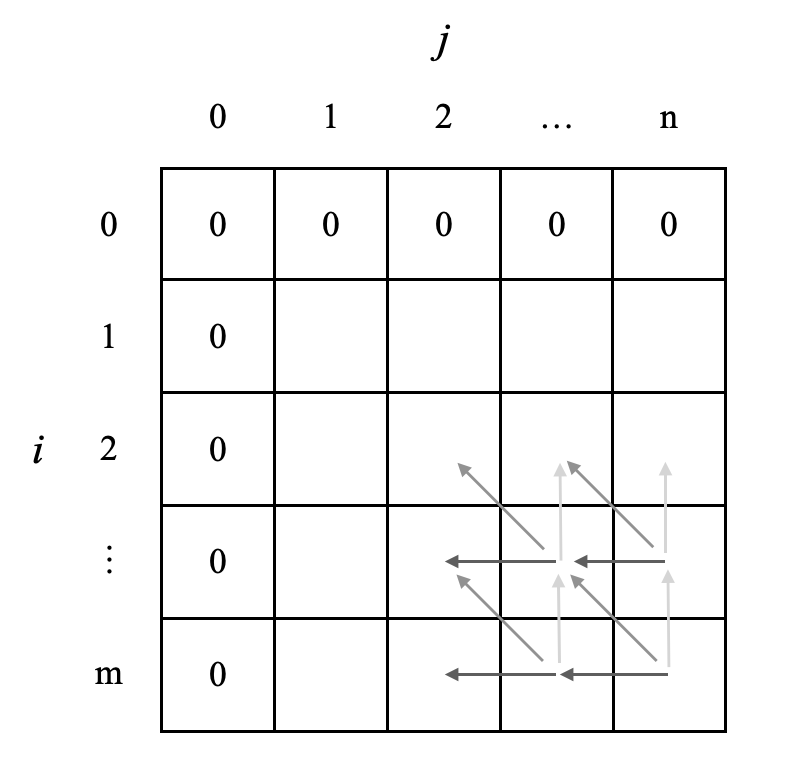
\includegraphics[scale=0.7]{hw5q6.png}

\item Compute the value of an optimal solution bottom-up:
\begin{algorithmic}[1]
\Function{LCS-Length}{$X$, $Y$}
	\State $m = X$.length
	\State $n = Y$.length
	\State let $C[0..m, 0..n]$ be a new table
	\For {$i = 0$ \textbf{to} $m$}
		\State $C[i, 0] = 0$
	\EndFor
	\For {$j = 0$ \textbf{to} $n$}
		\State $C[0, j] = 0$
	\EndFor
	\For {$i = 1$ \textbf{to} $m$}
		\For {$j = 1$ \textbf{to} $n$}
			\If {$x_i == y_j$}
				\State $C[i, j] = C[i - 1, j - 1] + 1$
			\ElsIf {$C[i - 1, j] \ge C[i, j - 1]$}
				\State $C[i, j] = C[i - 1, j]$
			\Else
				\State $C[i, j] = C[i, j - 1]$
			\EndIf
		\EndFor
	\EndFor
	\State \textbf{return} $C$
\EndFunction
\end{algorithmic}

\item Trace the optimal solution from the computed information:
\begin{algorithmic}[1]
\Function{Trace-LCS}{$X$, $Y$, $C$} \Comment{$C$ is the resulting matrix of \textproc{\textsc{LCS-Length}}(\textit{X}, \textit{Y})}
	\State $i = X$.length
	\State $j = Y$.length
	\State $k = C[i, j]$
	\State $\textit{ans} =$ array of zeros of size $k$
	\While {$i > 0$ and $j > 0$}
		\If {$x_i == y_j$} \Comment{when $x_i$ equals $y_j$, it is a part of the final LCS}
			\State $\textit{ans}[k] = x_i$
			\State $k = k - 1$
			\State $i = i - 1$
			\State $j = j - 1$
		\ElsIf {$C[i - 1, j] \ge C[i, j - 1]$}
			\State $i = i - 1$
		\Else
			\State $j = j - 1$
		\EndIf
	\EndWhile
	\State \textbf{return} \textit{ans}
\EndFunction
\end{algorithmic}
We walk through the $C$ table to trace an LCS of $X$ and $Y$ starting from $C[X.\text{length}, Y.\text{length}]$ to any $C[0, j]$ or $C[i, 0]$ by moving to smaller subproblems that yields a longer LCS.

\item Runtime and space requirements:

The runtime for \textproc{\textsc{LCS-Length}} is $O(mn)$ because the operations within the doubly-nested for loops are constant time. Its space requirement is also $O(mn)$ which is primary the $C$ table. To trace the solution, \textproc{\textsc{Trace-LCS}} runs in $O(m + n)$ time taking $O(k)$ spaces. Overall, the LCS problem can be solved in $O(mn)$-time.
\end{enumerate}

Initially, we create $Y$ that is a sorted copy of $X$, which takes $O(n\log n)$-time using merge sort. Now that the DP solution of LCS runs in $O(mn)$ time, and that $X$ and $Y$ are of the same size $n$, solving the problem takes $O(n^2)$-time.

\end{document}